% filepath: c:\Users\kuba-\Desktop\simple_graph_tool_xdf\src\eeg\reportPendulum.tex
\documentclass[12pt]{article}
\usepackage[T1]{fontenc} % Use T1 font encoding
\usepackage[utf8]{inputenc} % Ensure UTF-8 encoding
\usepackage[polish]{babel} % Enable Polish language support
\usepackage{amsmath}
\usepackage{graphicx}
\usepackage{booktabs}
\usepackage{float}
\usepackage[margin=2.5cm]{geometry}
\usepackage{siunitx}
\usepackage{titlesec}
\titlespacing*{\subsection}{0pt}{*0.5}{*0.5} % Adjusts spacing before and after subsections
\usepackage{caption}
\usepackage{lmodern}
\usepackage{placeins} % For FloatBarrier
\usepackage{hyperref} % For hyperlinks in the document

\title{Sprawozdanie z Laboratorium Fizyki: Wahadło fizyczne}
\date{}

\begin{document}

% --------------------------- STRONA TYTUŁOWA --------------------------
\begin{titlepage}
    \centering
    \Large
    \textbf{DYDAKTYCZNE LABORATORIUM FIZYKI} \\
    \vspace{0.2cm}
    \textbf{UNIWERSYTET RADOMSKI}\\
    im. Kazimierza Pułaskiego w Radomiu \\
    
    \vspace{1.5cm}
    \begin{flushleft}
        \textbf{Wydział:} {WTEiI} \\
        \textbf{Kierunek:} Informatyka \\
        \textbf{Rok Akademicki:} 2024/2025 \\
        \textbf{Semestr:} II \\
        \textbf{Grupa:} 3 \\
        \textbf{Zespół:} 2 \\
        \textbf{Data:} 11.03.2025 \\
        \textbf{Prowadzący ćwiczenie:} dr B. Winiarska \\
    \end{flushleft}
    
    \vspace{1cm}
    \begin{flushleft}
        \textbf{Nr ćwiczenia:} 2 \\
        \textbf{Temat ćwiczenia:} \\
        \textbf{Ruch Harmoniczny bryły (Wahadło fizyczne)} \\
    \end{flushleft}
    
    \vspace{1cm}
    \begin{flushleft}
        \textbf{Wykonujący ćwiczenie:}
        \begin{itemize}
            \item Jakub Oleszczuk
            \item Mikołaj Majewski
            \item Mateusz Ofiara
        \end{itemize}
    \end{flushleft}

    \vfill
    \begin{flushleft}
        \textbf{Oceny:} \\
        1.\hspace{2cm}2.\hspace{2cm}3.
    \end{flushleft}
\end{titlepage}

% --------------------------- TREŚĆ SPRAWOZDANIA --------------------------
\section*{Wstęp}

Celem ćwiczenia było eksperymentalne wyznaczenie przyspieszenia ziemskiego g z wykorzystaniem wahadła matematycznego. 
Badanie polegało na analizie ruchu drgającego harmonicznego poprzez pomiar okresu drgań dla różnych długości nici. 
Na podstawie zależności T. Okres T na potrzeby ćwiczenia został wyliczony jako: \[ T = 2\pi \sqrt{\frac{I}{mgd}} \] wykonano analizę regresji liniowej, 
umożliwiającą obliczenie wartości przyspieszenia ziemskiego.
Ćwiczenie miało również na celu lepsze zrozumienie zasad rządzących ruchem drgającym 
oraz nabycie praktycznych umiejętności związanych z pomiarami fizycznymi i opracowaniem danych eksperymentalnych.

\section*{Wyniki pomiarów}

\begin{itemize}
    \item Masa: \( m = 0.783 \, \text{kg} \)
    \item Długość pręta: \( l = 0.9 \, \text{m} \pm -0.1 \, \text{m} \)
    \item Środek ciężkości: \( s = 0.45 \, \text{m} \pm -0.1 \, \text{m} \)
    \item Wychylenie: \( \alpha = 15^\circ \pm 1^\circ \)
\end{itemize}

Tabela pomiarów (czas 20 drgań, 2 pomiarów dla różnych odległości od środka ciężkości pręta):

\begin{center}
    \begin{tabular}{|c|c|c|c|c|c|c|}
    \hline
    L.p. & d [m] & t1 [s] & t2 [s] & T [s] & X [m²] & Y [m$\cdot$s$^{-2}$] \\
    \hline
    1 & 0{,}35 & 28{,}91 & 28{,}90 & 1{,}45 & 0{,}010 & 0{,}21 \\
    2 & 0{,}32 & 28{,}58 & 29{,}11 & 1{,}44 & 0{,}017 & 0{,}27 \\
    3 & 0{,}29 & 28{,}79 & 28{,}80 & 1{,}44 & 0{,}026 & 0{,}33 \\
    4 & 0{,}26 & 29{,}21 & 28{,}93 & 1{,}45 & 0{,}036 & 0{,}40 \\
    5 & 0{,}23 & 29{,}26 & 29{,}39 & 1{,}47 & 0{,}048 & 0{,}47 \\
    6 & 0{,}20 & 30{,}71 & 30{,}44 & 1{,}53 & 0{,}063 & 0{,}58 \\
    7 & 0{,}17 & 31{,}24 & 31{,}47 & 1{,}57 & 0{,}078 & 0{,}69 \\
    8 & 0{,}14 & 34{,}24 & 34{,}04 & 1{,}71 & 0{,}096 & 0{,}90 \\
    9 & 0{,}11 & 38{,}17 & 38{,}19 & 1{,}91 & 0{,}116 & 1{,}24 \\
    10 & 0{,}08 & 48{,}26 & 48{,}38 & 2{,}42 & 0{,}137 & 2{,}16 \\
    \hline
    \end{tabular}
    \end{center}
    


\section*{Wykres}

\begin{figure}[H]
    \centering
    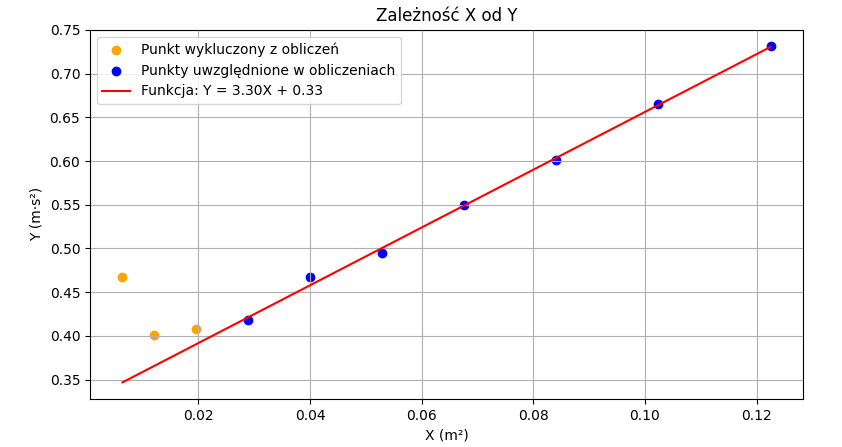
\includegraphics[width=0.8\textwidth]{pendulum.png}
    \caption{Wykres zależności \( \textbf{X} = d \) od \( \textbf{Y} = d \cdot T^2 \)}
    \label{fig:pendulum}
\end{figure}

\begin{raggedright}
{\small \textit{Kod źródłowy do podanego wyżej wykresu znajduje się na platformie github pod linkiem: \\ 
\url{https://github.com/scmisa/simple_graph_tool_xdf}}}
\end{raggedright}

\normalsize\normalfont

Na wykresie są przedstawione wszystkie punkty pomiarowe oraz linia regresji,
ale 3 punkty odstające (10, 9, 8) zostały usunięte z obliczeń, 
ponieważ ich wartości znacznie odbiegały od pozostałych pomiarów
powodując duże błędy w obliczeniach przyspieszenia ziemskiego
oraz momentu bezwładności.

\clearpage

\section*{Obliczenia}
Na podstawie pomiarów obliczono wartości \( X \) i \( Y \) dla każdego pomiaru. 
Następnie obliczono średnie wartości \( \bar{X} \) i \( \bar{Y} \)
oraz Metodą Najmniejszych Kwadratów wyznaczono współczynniki \( A \) i \( B \)
w celu obliczenia przyspieszenia ziemskiego \( g \) oraz momentu bezwładności \( I_0 \)
z wzorów:

\begin{align*}
X &= d, \quad Y = d \cdot T^2 \\
\bar{X} &= \frac{\sum X_i}{n}, \quad \bar{Y} = \frac{\sum Y_i}{n} \\
A &= \frac{4\pi^2}{g} ,\quad B = \frac{4\pi^2 \cdot I_o}{m \cdot g} \\
u(A) &= \sqrt{\frac{1}{n-2} \cdot \frac{\sum (Y_i - A \cdot X_i - B)^2}{\sum (X_i - \bar{X})^2}} \\
u(B) &= u(A) \cdot \sqrt{\frac{\sum X_i^2}{n}} \\
g &= \frac{g}{4\pi^2} \\
u(g) &= \frac{g}{A} \cdot u(A) \\
I_0 &= m \cdot \frac{B}{A} \\
u(I_0) &= I_0 \sqrt{\left(\frac{u(A)}{A}\right)^2 + \left(\frac{u(B)}{B}\right)^2}
\end{align*}

Wzory na współczynniki regresji liniowej:
\begin{align*}
A &= \frac{\sum (X_i - \bar{X})(Y_i - \bar{Y})}{\sum (X_i - \bar{X})^2} \\
B &= \bar{Y} - A \cdot \bar{X} \\
\end{align*}


Po dopasowaniu prostej uzyskano:
\[
A = 3.30 \pm 0.07 \, \mathrm{s^2/m}, \quad B = 0.33 \pm 0.01 \, \mathrm{m/s^2}
\]

Wartość \( g \) została obliczona jako:
\[
g = 11.95 \pm 0.78 \, \mathrm{m/s^2}
\]

Moment bezwładności został obliczony jako:
\[
I_0 = 0.7720 \pm 0.0019 \, \mathrm{kg \cdot m^2}
\]


\clearpage

\section*{Wnioski}

\subsection*{Przyczyny systematycznych niepewności pomiarowych}
Podczas wykonywania ćwiczenia zdarzało się iż nasze dwa tak samo wykonane pomiary osiągały rozbieżne wyniki 
które nie są brane pod uwagę w tym wypracowaniu ponieważ przekraczają one dozwolony błąd pomiarowy. 
Jest to spowodowane dlatego, że pomiary wykonywaliśmy stoperem oraz własnymi obserwacjami używając wzroku. 
Stoper posiada swoje własne opóźnienie poprzez swój mechanizm, jednakże głównym czynnikiem niepewności jest nasz czas reakcji.



\subsection*{Dokładność metody wyznaczania przyspieszenia ziemskiego}
 Obliczona wartość g nie była zbliżona do wartości teoretycznej (ok. 9.81 m/s²) wynikające z niedokładności wykonania pomiarów przez studentów.


 \subsection*{Możliwości poprawy dokładności pomiarów}
 Aby zredukować błędy systematyczne, w przyszłości można zastosować bramki optyczne zamiast ręcznego pomiaru czasu stoperem, co wyeliminuje wpływ czasu reakcji obserwatora.


\subsection*{Wpływ wykluczenia punktów odstających}
 W celu poprawy jakości analizy został wykluczony jeden punkt o znacznym błędzie, co pozwoliło uzyskać bardziej wiarygodne wyniki regresji liniowej.


\end{document}
